\subsection{wiringPi}
Auf dem Rapberry Pi 4 ist die  wiringPi Libarry vorinstalliert. 
Die Funktionalität der drei verwendeten C-Funktionen wird im folgenden beschrieben.

\subsubsection{wiringPiI2CSetup}
Der Funktion wird beim Aufruf die I2C Adresse übergeben mit welcher eine Verbindung aufgebaut werden soll: $wiringPiI2CSetup(address)$.\\
Der Rückgabewert ist der Standard Linux File Descriptor oder -1, falls ein Fehler auftritt. 
Die Anzahl der File Desciptoren ist begrenzt daher muss die Verbindung mit der Funktion $close()$ aus der Library: unistd.h geschlossen werden wenn sie nicht mehr benötigt wird.

\subsubsection{wiringPiI2CWriteReg8}
Der Funktion wird beim Aufruf der File Descriptor einer aktiven I2C Verbindung sowie ein Zielregister und die zu schreibenden 8bit Daten übergeben:\\ $wiringPiI2CWriteReg8 (fd, RegAdr, 8BitData)$.
Wenn der Schreibzugriff vom I2C gerät bestätigt wurde wird eine 0 zurück gegeben.
\subsubsection{wiringPi4I2CReadReg8}
Der Funktion wird beim Aufruf der File Descriptor einer aktiven I2C Verbindung sowie ein Zielregister übergeben: $wiringPiI2CReadReg8(fd, RegAdr)$.
Der gelesene 8-Bit-Inhalt des Registers ist der Rückgabewert.
Wenn das Lesen Fehlschlägt bleibt das Programm in einer Endlosschleife hängen.

\subsection{AS726X Libary}
Die WiringPi\_AS726X\_Libary enthält alle Funktionen um den AS7261 und AS7265X zu steuern und auszulesen.
Da der Beispiel Code und die sonstigen Angaben im Datenblatt in vielen Detailfragen ungenau und Fehlerhaft sind wurde die Arduino OpenSource Libarrys von sparkfun SparkFun\_AS726X\_Arduino\_Library-master und SparkFun\_AS7265x\_Arduino\_Library als Implementierungsgrundlage verwendet.
Im ersten schritt der Entwicklung wurde sie für die I2C Schnittstelle, wiringPi Libarry des Rapberry Pi 4 umgeschrieben und anschließen in ihrer Funktionalität erweitert um für das Messystem mit mehreren Sensoren auf dem gleichen I2C-Bus nutzbar zu sein. \\

Im Folgenden Text werden die Register Adressen und mit den gleichen Namen wie im source code bezeichnet die Numerische Adressen sind in Tabelle \ref{TODO} aufgelistet. TODO table

\begin{figure}[H]
\centering
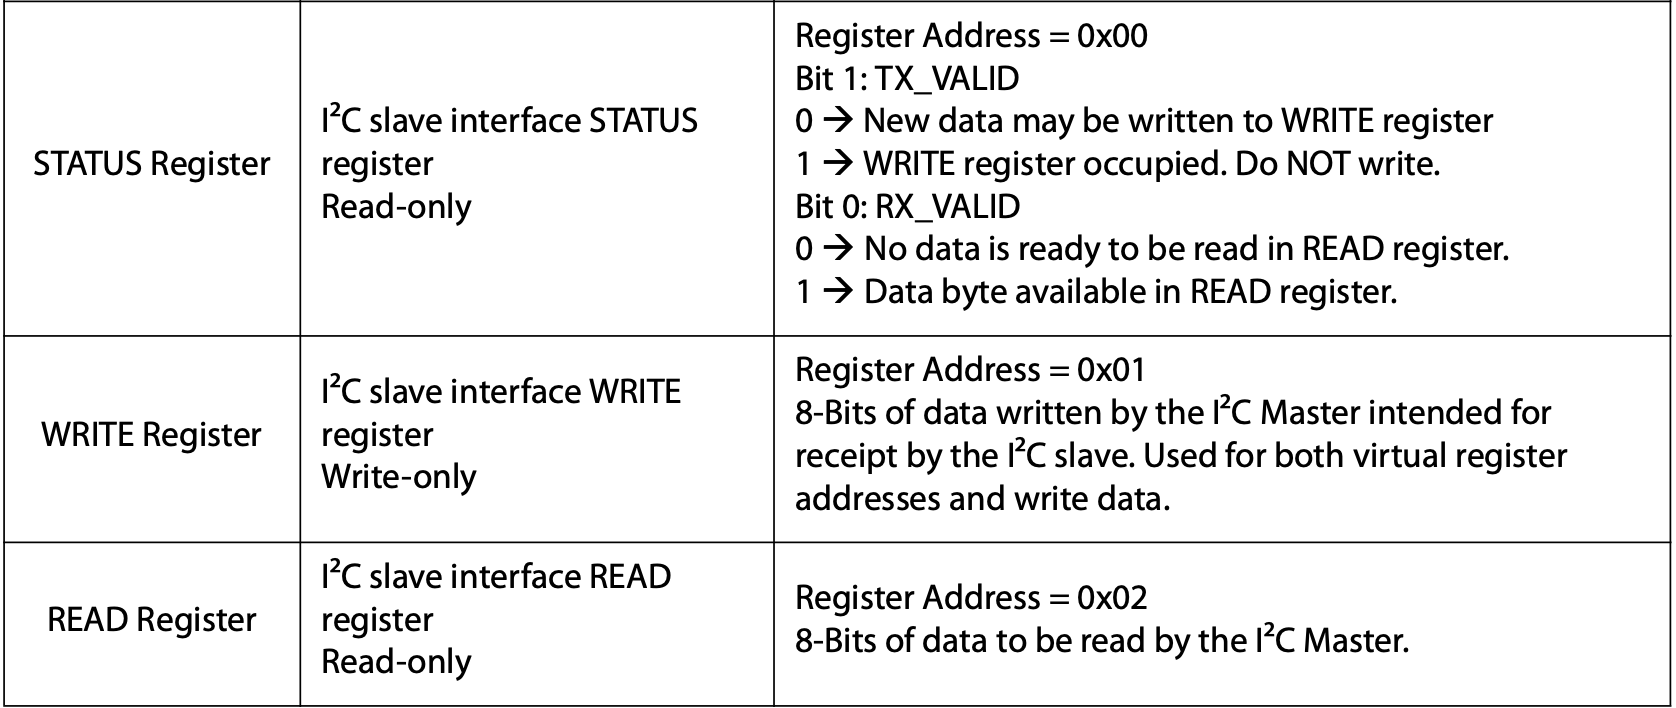
\includegraphics[width=0.75\textwidth]{img/PysicalRegister}
%\caption*{Quelle: Datenblatt AS7261}
\caption{PysicalRegister}
\label{fig:PysicalRegister}
\end{figure}

\begin{figure}[H]
\centering
\caption{AS726x\_CONTROL\_SETUP 0x04}
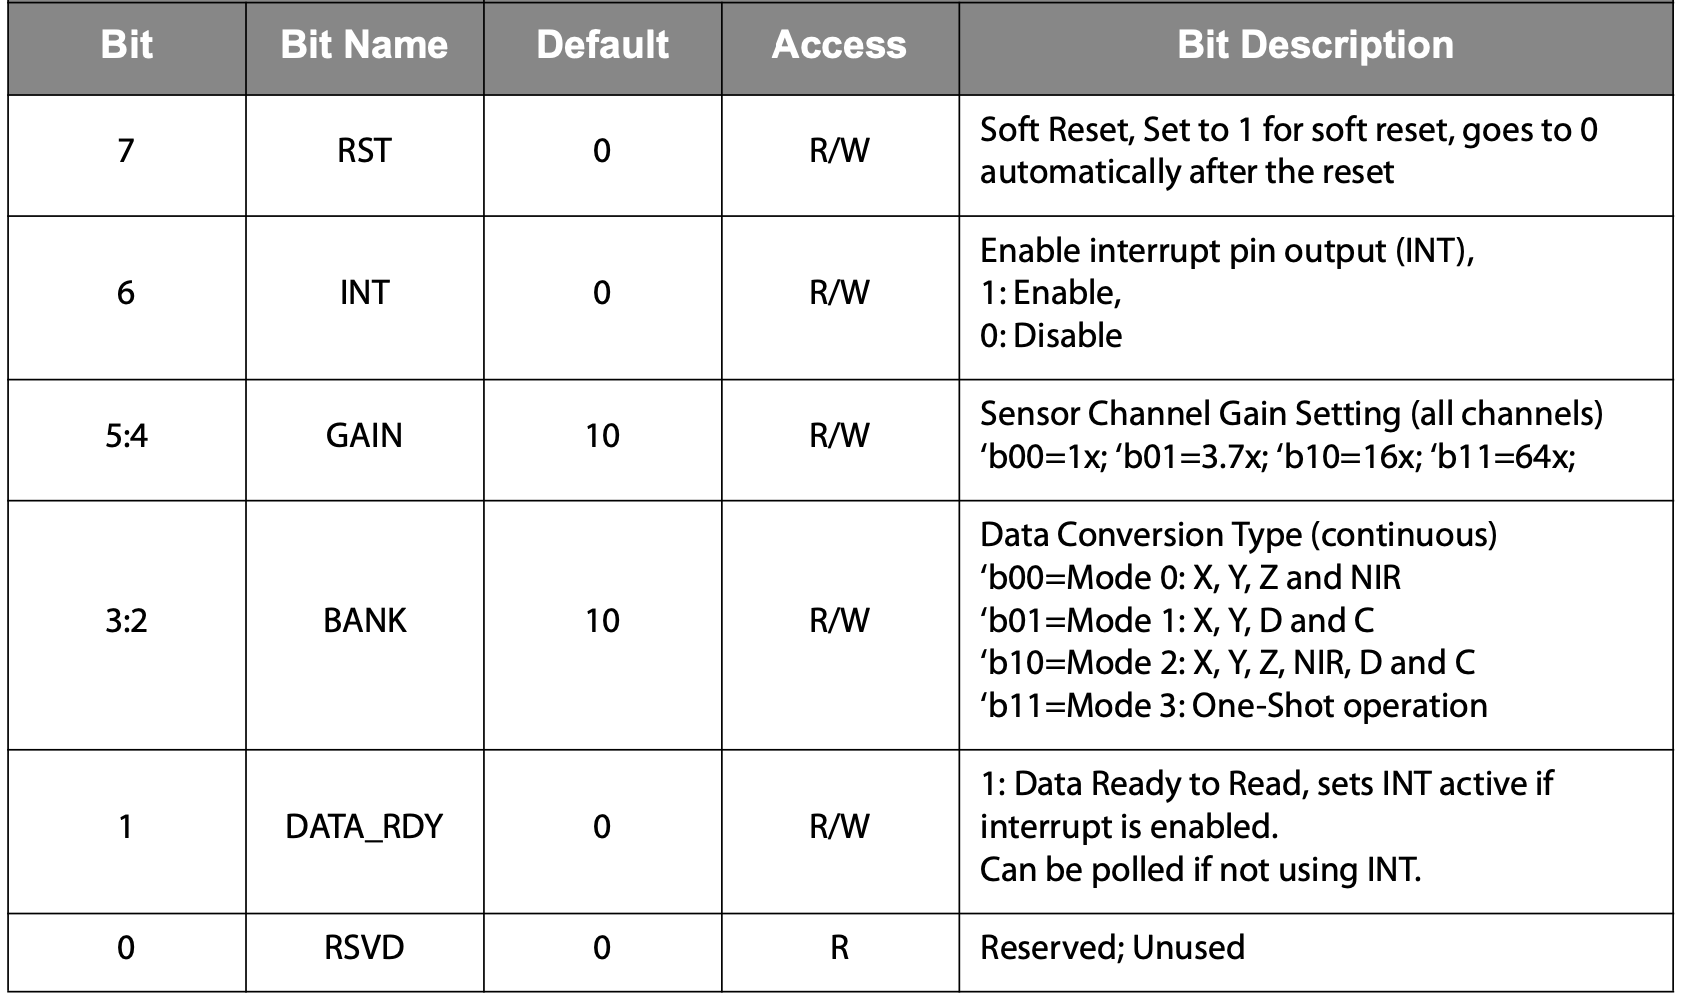
\includegraphics[width=0.75\textwidth]{img/AS726x_CONTROL_SETUP}
\caption*{Quelle: Datenblatt AS7261}
\label{fig:AS726x_CONTROL_SETUP}
\end{figure}

\begin{figure}[H]
\centering
\caption{AS726x\_INT\_T 0x05}
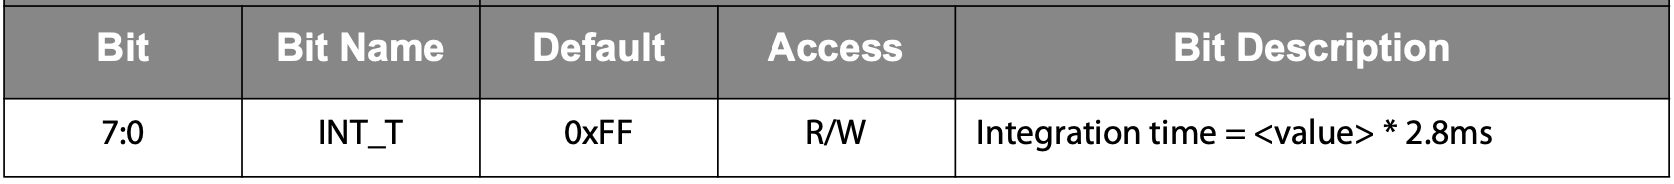
\includegraphics[width=0.75\textwidth]{img/AS726x_INT_T}
\caption*{Quelle: Datenblatt AS7261}
\label{fig:AS726x_INT_T}
\end{figure}

\begin{figure}[H]
\centering
\caption{AS726x\_DEVICE\_TEMP 0x06}
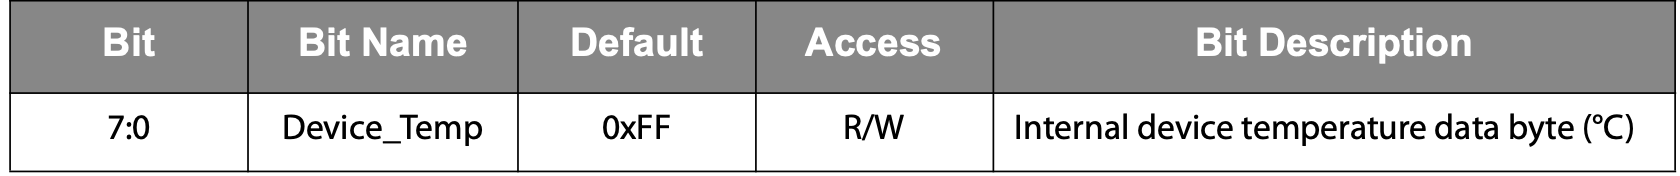
\includegraphics[width=0.75\textwidth]{img/AS726x_DEVICE_TEMP}
\caption*{Quelle: Datenblatt AS7261}
\label{fig:AS726x_DEVICE_TEMP}
\end{figure}

\begin{figure}[H]
\centering
\caption{AS726x\_LED\_CONTROL 0x07}
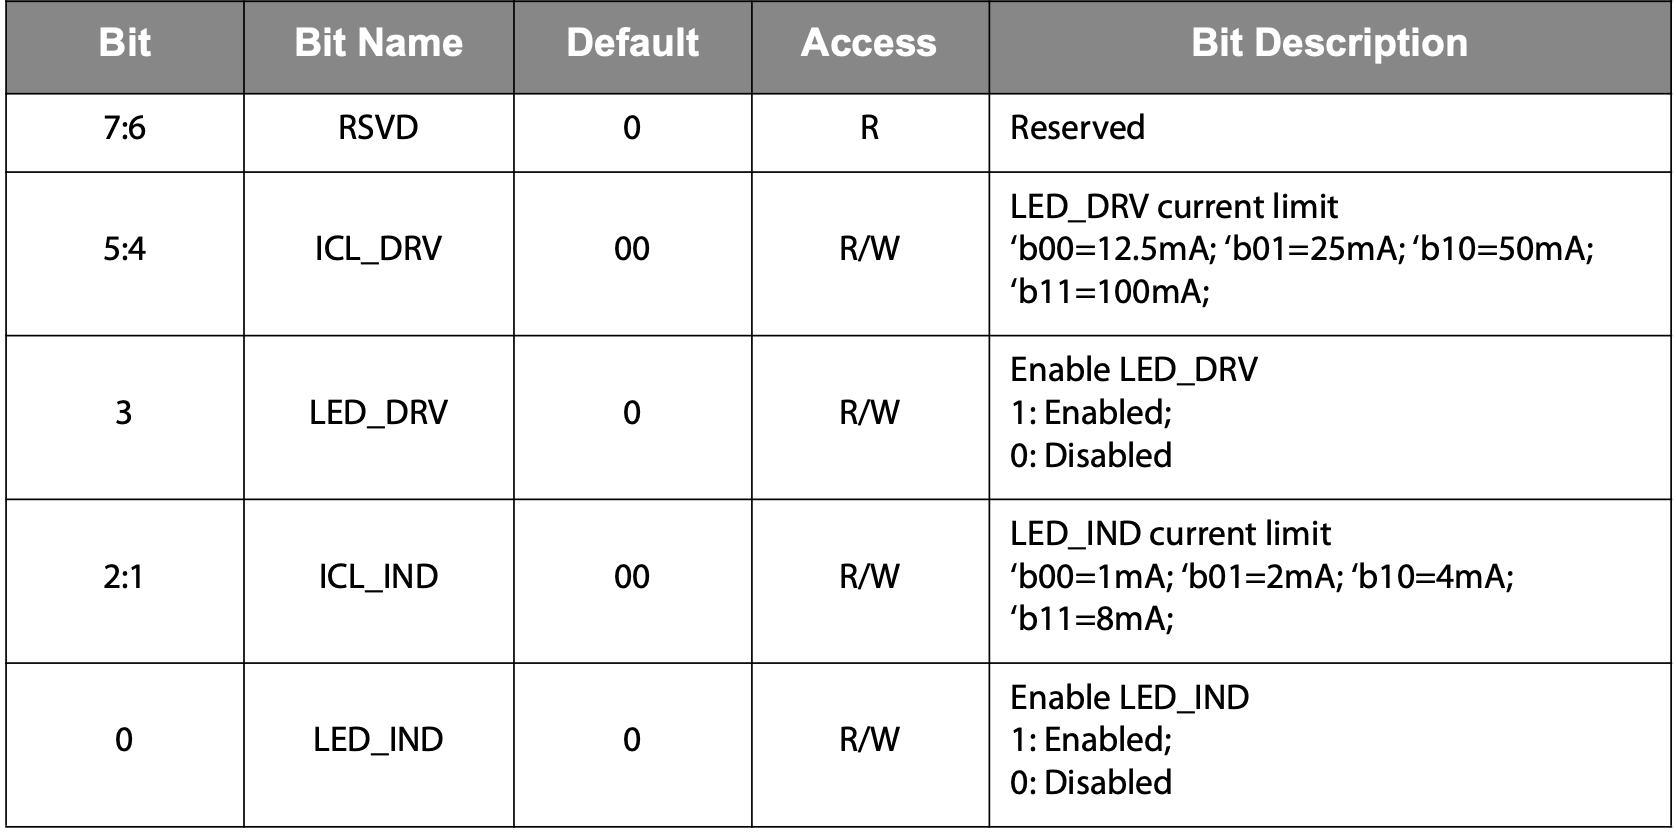
\includegraphics[width=0.75\textwidth]{img/AS726x_LED_CONTROL}
\caption*{Quelle: Datenblatt AS7261}
\label{fig:AS726x_LED_CONTROL}
\end{figure}

\begin{figure}[H]
\centering
\caption{AS7265X\_DEV\_SELECT\_CONTROL 0x4F}
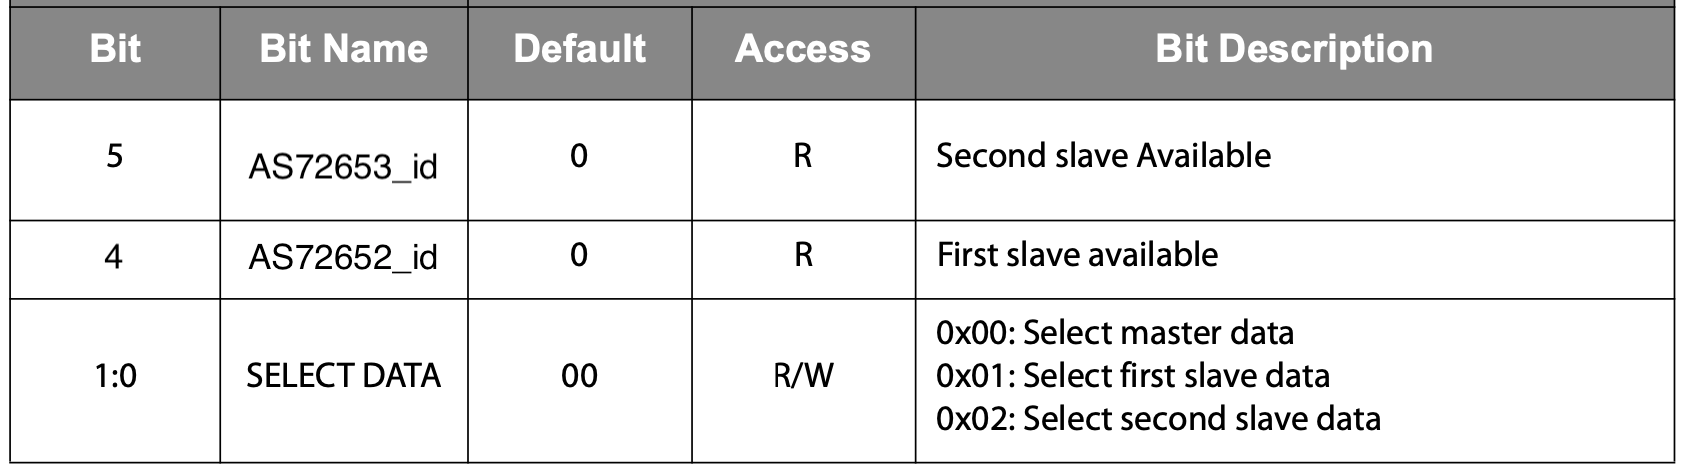
\includegraphics[width=0.75\textwidth]{img/AS7265X_DEV_SELECT_CONTROL}
\caption*{Quelle: Datenblatt AS7265X}
\label{fig:AS7265X_DEV_SELECT_CONTROL}
\end{figure}

\begin{table}[!ht]
\centering
\caption{Raw Data Channel Registers}
\begin{tabular}{ l r }
 Name & Adresse\\ 
AS7261\_X & 0x08\\
AS7261\_Y & 0x0A\\
AS7261\_Z & 0x0C\\
AS7261\_NIR & 0x0E\\
AS7261\_DARK & 0x10\\
AS7261\_CLEAR & 0x12\\
AS7265X\_R\_G\_A & 0x08 \\
AS7265X\_S\_H\_B & 0x0A \\
AS7265X\_T\_I\_C & 0x0C \\
AS7265X\_U\_J\_D & 0x0E \\
AS7265X\_V\_K\_E & 0x10 \\
AS7265X\_W\_L\_F & 0x12 \\
\end{tabular}
\label{fig:raw_channel_registers}
\end{table}

\subsubsection{virtualWriteRegister}
Wie bei Embedded-Geräten üblich werden Einstellungen auf dem Sensor verändern indem verschiedene sogenannte Special Function Register mit Daten beschrieben werden.\\
Jedes Special Function Register ist 8Bit groß und hat eine Adresse. Jedes Bit des Register repräsentiert eine Einstellung.
Beispielsweise ist 0x07 (Abb. \ref{fig:AS726x_LED_CONTROL}) das LED Control Register des Sensors.
Bit 0 des Registers Beschreibt den Zustand der Status LED.
Die Restlichen 7 Bit des Registers Beschreibt den Zustand anderer LEDs die für den Messaufbau aber irrelevant sind.\\
Wird Register 7 mit dem Dezimalwert 0 beschrieben sind alle LED aus, wird es mit dem Dezimalwert 1 beschrieben leuchtet nur die Status LED.
Die Register Lassen sich aber nicht direkt Beschreiben, stattdessen sind sie als sogenannte Virtuelle Register Implementiert.
Das heißt das nur Register 0x01 (WRITE Register Abb. \ref{fig:PysicalRegister}) beschrieben werden kann.
Um Daten in eins der Special Funktion Register zu schreiben wird die C-Funktion virtualWriteRegister verwendet.
Die Funktionsweise lässt sich in 4 schritten zusammenfassen:
\begin{itemize}
	\item Zeile 8 wartet bis das WRITE Register leer ist, was angezeigt wird indem  das Bit AS72XX\_TX\_VALID im  Register AS72XX\_STATUS\_REG den Wert 1 annimmt.
	\item Zeile 14 Schreibt die Virtuelle Adresse in das WRITE Register und Setzt zusätzlich Bit 8 des WRITE Register auf 1 um zu zeigen das es sich um einen Schreibenden zugriff auf das Virtuelle Register handelt.
	\item Zeile 20 wartet erneut bis das WRITE Register leer ist.
	\item Zeile 26 schreibt die Daten in das WRITE Register
\end{itemize}
Der Sensor wird jetzt selber die übertragenen Daten aus dem WRITE Register in das angegebene Virtuelle Register kopieren.
\lstinputlisting[language=C,style=c]{code/virtualWriteRegister.c}

\subsubsection{virtualReadRegister}
Die Unterschiedlichen Messdaten des Sensors werden in dedizierten Registern gespeichert.
 Es ist aber nur über den indirekten weg des AS72XX\_READ\_REG und der Virtuellen Register Adressen möglich Daten auszulesen.
Die Funktionsweise der zum Daten auslesen benötigten Funktion virtualReadRegister lässt sich wieder in 4 Schritte aufteilen.
\begin{itemize}
	\item Das AS72XX\_READ\_REG wird ausgelesen ohne das die Daten verarbeitet werden. Dieser schritt ist wie ein Reset des Registers zu verstehen.
	\item Zeile 12 schreibt die Virtuelle Adresse in das WRITE Register und setzt zusätzlich Bit 8 des WRITE Register auf 0 um zu zeigen das es sich um einen Lesenden zugriff auf das Virtuelle Register handelt.
	\item Sobald das AS72XX\_STATUS\_REG den Wert AS72XX\_TX\_VALID annimmt sind die Daten aus dem angebenden Virtuellen Register in das AS72XX\_READ\_REG kopiert worden.
	\item Zeile 28 liest die Daten aus dem S72XX\_READ\_REG
\end{itemize}
\lstinputlisting[language=C,style=c]{code/virtualReadRegister.c}

\subsubsection{MeasurementFromAdress}
Die Funktion baut einen I2C Verbindung zur übergebenen Bus-Adresse auf und  ruft die Funktion takeMeasurments mit dem File Descriptor der aktiven I2C Verbindung auf.
Nachdem die Funktion takeMeasurements durchlaufen ist wird die I2C Verbindung wieder geschlossen.
\lstinputlisting[language=C,style=c]{code/MeasurementFromAdress.c}

\subsubsection{takeMeasurements}

Die Funktion takeMeasurements ruft die Funktion setMeasurementMode mit dem Parameter 3 auf das setzt den aus \ref{todo} bekannten Bankmode der übergebenen I2C Verbindung (fd) auf Bank Mode 3.
	Die On-Shot Messung wird sofort gestartet, in Zeile 9 wird gewartet bis die Messung abgeschlossen ist. 
		Um sicherzustellen das die Funktion DataAvailable richtig arbeitet muss vor der Messung das Flag DataAvailable auf 0 gesetzt werden (Zeile 3).
Die Daten werden hier nicht ausgelesen daher gibt es keinen Rückgabewert.\\
\lstinputlisting[language=C,style=c]{code/takeMeasurements.c}

\subsubsection{setMeasurementMode}
Mit der Funktion setMeasurementMode werden die Bankmode Bits 2 und 3 des \\
AS726x\_CONTROL\_SETUP Registers mit dem gewünschten Wert für den Bankmode beschrieben.\\
Da die anderen Bits des Registers noch weitere Einstellungen repräsentieren welche nicht verändert werden sollen, muss das Register erst ausgelesen werden.
Anschließend werden die Bankmode Bits auf 0 gesetzt um im nächsten schritt mit dem gewünschten neuen Bankmodewert beschrieben zu werden. 
Die Bedeutung der Bankmodes ist in \ref{TODO} erläuteret.
\lstinputlisting[language=C,style=c]{code/setMeasurementMode.c}
\subsubsection{dataAvailable \& clearDataAvailable}
Das Bit dataAvailble im Register AS726x\_Control\_Setup wird vom Sensor auf 1 gesetzt wenn nach einer Messung neue Daten vorhanden sind, Interrupts müssen dafür ausgeschaltet sein.
dataAvailble wird auf 0 gesetzt wenn Daten gelesen werden.
Wenn eine One-Shot Messung im Bankmode 3 durchgeführt wird muss das dataAvailble Bit mit der Funktion clearDataAvailable auf 0 gesetzt werden, da sonst nicht sicher gestellt ist das die Daten vor der Messung gelesen wurden besteht die Möglichkeit das sich das Bit fälschlicherweise noch im falsch positiven zustand befindet.
Die Funktion dataAvailable gibt den Wert des DataAvailable Bit zurück.\\

%\lstinputlisting[language=C,style=c]{code/dataAvailable.c}

\subsubsection{Rohwerte des AS7261 Auslesen}
Die in \ref{todo} beschrieben 6 Channel des AS7261 werden mit den folgenden Funktionen ausgelesen:
\begin{itemize}
	\item getX\_CIE(fd)
	\item getY\_CIE(fd)
	\item getZ\_CIE(fd)
	\item getNIR(fd)
	\item getDark(fd) 
	\item getClear(fd)
\end{itemize}
Der File Deskriptor einer I2C Verbindung mit einem AS7261 und das zu lesende Register(Abb. \ref{fig:raw_channel_registers}) wird als Übergabe Parameter erwartet.\\
Um den Messwert auszulesen, wir die Funktion getchannel aufgerufen.
Der Rückgabewert ist der 16-Bit Messwert aus dem jeweiligen Register vom Datentyp integer.
\lstinputlisting[language=C,style=c]{code/getRaw_AS7261.c}

\subsubsection{getChannel}
Da die Messdaten 16-Bit groß sind, der Sensor aber nur über 8 Bit Register verfügt werden 2 aufeinader folgende Register ausgelsen und im Big-Endian Format aneinander geheftet.
Die Funktion getChannel erwartet den File Descriptor einer I2C Verbindung zu einem Sensor und die Adressen des High Bytes eines Raw Data Registers.
Der Rückgabewert ist der 16-Bit Messwert aus dem jeweiligen Register vom Datentyp Integer.\\

\lstinputlisting[language=C,style=c]{code/getChannel.c}

\subsubsection{Rohwerte des AS7265X Auslesen}
Da beim lesen des AS7265X, 3 Sensoren unter der gleichen Adresse erreichbar sind (Abb. \ref{fig:raw_channel_registers}), muss zusätzlich zum File Disciptor und des ziel Registers der Device Identifier angeben werden.
Die folgenden Funktionen übernehmen diese Aufgaben und können genutzt werden, um Rohdaten auslesen:
\begin{center}
\begin{tabular}{ c c c }
 	AS72651 & AS72652 & AS72653 \\ 
 	getR(fd) & getG(fd) & getA(fd) \\  
 	getS(fd) & getX(fd) & getB(fd) \\
 	getT(fd) & getI(fd) & getC(fd) \\  
 	getU(fd) & getJ(fd) & getD(fd) \\
 	getV(fd) & getK(fd) & getE(fd) \\  
 	getW(fd) & getL(fd) & getF(fd) \\
\end{tabular}
\end{center}
Um den Messwert auszulesen, wir die Funktion getChannel\_AS7265X aufgerufen.\\
Der Rückgabewert ist der 16-Bit Messwert aus dem jeweiligen Register vom Datentyp integer.\\

%\lstinputlisting[language=C,style=c]{code/getRaw_AS7265X.c}

\subsubsection{getChannel\_AS7265X}
Die Funktion verarbeitet den aus \ref{Rohwerte des AS7265X Auslesen} bekannten Device Identifier indem die Funktion selectDevice aufgerufen wird.
	Da es aber keine Möglichkeit gibt zu überprüfen ob der Gerätewechsel erfolgreich war muss vorher überprüft werden ob das jeweiligen Slavegerät AS72652 oder AS72653 vorhanden ist.
	Ist ein Slave nicht vorhanden wird der Wert -1 zurück gegeben.
	Ohne diese Überprüfung ist nicht sichergestellt das keine falschen Werte aus den gleich nummerierten Registern des AS72651 ausgelesen werden, obwohl Werte eines nicht vorhandnen oder falsch aufgelöteten Slavesensors (AS72652 / AS72653)erwartet werden.
	Das eigentliche auslesen des 16-Bit Messwerts erfolgt mithilfe der Funktion getChannel, das Ergebnis ist der Rückgabewert der Funktion getChannel\_AS7265X.\\

\lstinputlisting[language=C,style=c]{code/getChannel_AS7265X.c}

\subsubsection{selectDevice}
Die Notwendigkeit für selectDevice wurde in \ref{getChannel_AS7265X} bereits erläutert.
Laut Datenblatt sollen nur die Bits 0 und 1 des DEV\_SELECT\_CONTROL Registers beschrieben werden, das stimmt aber nicht.\\
In der Realität muss das gesamte 8-bit Register mit folgenden Werten beschrieben werden um beim anschließenden Lesevorgang Daten vom jeweiligen Sensor zu erhalten.
\begin{center}
\begin{tabular}{ c c }
 	DEV\_SELECT\_CONTROL & Sensor \\ 
 	0x00 & AS72651 \\  
 	0x01 & AS72652 \\
 	0x02 & AS72653 \\  
\end{tabular}
\end{center}

\lstinputlisting[language=C,style=c]{code/selectDevice.c}

\subsubsection{Enable/Disable Indicator}
Mit der Funktion enableIndicator wird das 0 Bit des AS726x\_LED\_CONTROL Register aus 1 gesetzt, so wird die Rote Status LED des jeweiligen Sensors auf dem Sensorboard angeschaltet.\\
Mit der Funktion disableIndicator wird das gleiche Bit auf 0 gesetzt, also die Led ausgeschaltet.\\
Als Übergabeparameter wird bei beiden Funktionen der File Diskiptor einer aktiven I2C-Verbindung erwartet.\\

%\lstinputlisting[language=C,style=c]{code/enableIndicator.c}

\subsubsection{softReset}
Der Sensor liefert in einigen Situationen Messwerte außerhalb des Erwartungsbereiches.
Dieses Problem kann in manchen fällen behoben werden indem ein softReset durchgeführt wird.
Da bei der hier beschriebenen Implementierung keine Fehler auftreten, wird die Funktion nicht benötigt, kann aber in zukünftigen Versionen verwendet werden.

Die Funktion softReset setzt das 8 Bit des Registers CONTROL\_SETUP auf 1 um einen softReset auszulösen.
Das Datenblatt gibt an, das mindestens 1000 ms gewatet werden muss, bevor der softReset abgeschlossen ist und der Sensor wieder genutzt werden kann.
Für beide Funktionen wird der FileDiskiptor einer aktiven I2C-Verbindung als Übertragungsparameter erwartet.\\

%\lstinputlisting[language=C,style=c]{code/softReset.c}

\subsubsection{I2CScan}
Die Funktion I2CScan wird zu Beginn des Programms aufgerufen, um festzustellen, welche Sensoren an den I2C DataBus angeschlossen sind.
Die gefundenen Sensoradressen und der Sensortyp werden in das Struct sensor\_list geschrieben.\\
Die Adressen werden außerdem im Terminal angezeigt, so dass der Benutzer überprüfen kann, ob alle erwarteten Sensoren erkannt werden.
Als Übergabeparameter wird im call by refrence style ein Pointer zu einem Struct vom Typ sensor\_list erwartet.
Da die Daten direkt in das extern deklarierte(?) Struct geschrieben werden gibt es keinen Rückgabewert.
Um die angeschlossenen Sensoren zu detektieren wir zu jeder der $2^8$ möglichen I2C Adressen eine Verbindung aufgebaut und ein Schreibversuch mithilfe der Funktion wiringPiI2CWriteReg8 vorgenommen.
Wenn die Funktioon wiringPiI2CWriteReg8 eine 0 zurück gibt war der Schreibversuch erfolgreich also muss ein Sensor unter dieser Adresse vorhanden sein.
Das im Datenblatt nicht erwähnte Register mit der Adresse 0x05 wurde ausgewählt da es mit dem Wert 0x01 beschrieben werden kann ohne das der Sensor sein verhalten verändert.
Die Funktion getVersion wird genutzt um die Version des gefunden Sensors zu ermitteln.
Wenn ein AS72651 erkannt wird zusätzlich abgefragt ob auch die Slavesensoren AS72652 und AS72653 vorhanden sind, diese Information wird nur im Terminal ausgegeben und nicht is das struct sensor\_list geschrieben, da es für den Programmablauf nicht notwendig ist.\\

\lstinputlisting[language=C,style=c]{code/I2C_Scan.c}

\subsubsection{getVersion}
Die Funktion getVersion gibt den Inhalt der Registers AS726x\_HW\_VERSION zurück, indem der zurückgegebene Wert mit den beiden SENSORTYPE Werten verglichen wird(SENSORTYPE\_AS7261 und SENSORTYPE\_AS72651) kann festgestellt werden um welchen Sensor es sich handelt. 
Als Übergabeparameter wird bei beiden Funktionen der File Diskiptor einer aktiven I2C-Verbindung erwartet.

\subsubsection{scanAS7262}
Als Übergabeparameter wird bei der Funktionen der FileDiskiptor einer aktiven I2C Verbindung mit einem AS72651 erwartet.\\
Die Funktion überprüft den Status des 4. Bit des Registers DEV\_SELECT\_CONTROL und gibt ihn zurück. Das Bit ist auf 1 gesetzt wenn der Slavesensor AS7262 vorhanden ist, im falle der Abwesenheit ist es 0.\\
Das AS7265X-Datenblatt gibt fälschlicherweise an, dass das 5. Bit geprüft werden muss.\\

\subsubsection{scanAS7263}
Als Übergabeparameter wird bei der Funktionen der FileDiskiptor einer aktiven I2C Verbindung mit einem AS72651 erwartet.\\
Die Funktion überprüft den Status des 5. Bit des Registers DEV\_SELECT\_CONTROL und gibt ihn zurück. Das Bit ist auf 1 gesetzt wenn der Slavesensor AS7263 vorhanden ist, im falle der Abwesenheit ist es 0.\\

\subsubsection{setGain}
Die Messergebnisse der Sensoren können intern verstärkt werden, was z.B. in dunklen Messumgebungen oder bei der Verwendung relativ lichtundurchlässiger Streuscheibe notwendig ist.\\
Außerdem kann das Speicherregister besser ausgelastet werden, um ein genaueres Messergebnis zu erhalten.
Um den Verstärkungsfaktor einzustellen, wird die Funktion setGain benötigt.\\
Die Funktion setGain beschreibt das 4 und 5 Bit des Registers CONTROL\_SETUP mit einem der 4 möglichen Zustände welcher an die Funktion sie übergebenen wird.

\begin{tabular}{ l l}
 	Wert & Verstärkungsfaktor \\ 
 	0 & 1x (power-on default) \\  
 	1 & 3.7x \\
 	2 & 16x \\  
 	3 & 64x \\
\end{tabular}

Ist der übergebe Wert größer als 3 ist wird das Register auf den Wert 3 gesetzt.

\subsubsection{setIntegrationTime}
Um die Integrationszeit der Messung einzustellen wird in das Register AS726x\_INT\_T ein Wert (integrationValue) zwischen 0 und 255 geschrieben, die Integrationszeit errechnet sich indem dieser Wert mit dem Faktor 2.8ms multipliziert wird.
Die Funktion setIntegrationTime erwartet als Übergabeparameter das integrationValue und den FileDiskiptor sowie eine aktive I2C-Verbindung zu einem Sensor.\\

\subsubsection{disableInterrupt}
Die Funktion disableInterrupt setzt das INT Bit im Register AS726x\_CONTROL\_SETUP auf 0 um Interrupts aus zu schalten.
Da der Interrupt-Pin auf der Sensor-Platine nicht angeschlossen ist, können Messungen nur durchgeführt werden, wenn der Interrupt ausgeschaltet ist.
Laut Datenblatt wird der Interrupt beim Systemstart ausgeschaltet.

\subsection{influxDB Library writeToDatabase}
Um die Messdaten der Sensoren in die aus \ref{datenbankundinterface} bekannte InfluxDB zu schreiben wurde die InfluxDB Library entwickelt, sie enthält nur eine einzige nach außen sichtbare Funktion: writeToDatabase.
\subsubsection{writeToDatabase}
Um die Datenbank zu beschreiben muss zuerst ein Socket geöffnet werden um sich mit der InfluxDB Server-Instanz  zu verbinden.
der InfluxDB Sever ist unter der Localhostaddress 127.0.0.1 am Port 8086 zu erreichen.
	Diese Werte können in der influxdb.h Datei angepasst werden falls in Zukunft die Notwendigkeit besteht den Server auf einem externen Gerät zu betreiben.\\
Die Kommunikation mit dem InfluxDB Server erfolgt über das Http basierte InfluxDB line protocol.
In Zeile 68 wird der Datenbankname , Username,  Passoword der Datenbank und die Größe des Body's der Anfrage in den Header teil der http anfrage geschrieben.
In Zeile 64 wird der Body teil der anfrage im InfluxDB line protocol Format erzeugt, dieser enthält den Bezeichner des Messwerts (z.B. X oder Y), die I2C Adresse des jeweiligen Sensors von dem die Messdaten stammen, den Messwert selbst sowie den Zeitstempel der Messung in ms.	
In Zeile 85 wird der Http request bestehend aus Header und Body an den Server übertragen.
Die Antwort vom Server wird gespeichert und anschließen auf die erwartete Rückmeldung "HTTP/1.1 204 No Content" untersucht, wenn der Schreibversuch fehlschlägt wird eine Meldung im Terminal angezeigt(TODO hier sollte die Status LED sich verändern).
\subsection{main}
In der Mainfunktion kommen 
\subsubsection{changeSettings}
TODO
\subsubsection{printTime}
TODO
\subsubsection{delayMeasurementMin}
TODO
\subsubsection{currentTimestamp}
TODO
\subsection{measurement}
TODO
\subsubsection{settings}
TODO
\subsubsection{matchValueToMaxGain}
TODO
\subsubsection{cleanAS7261Data}
TODO
\subsubsection{cleanAS7265XData}
TODO
\subsubsection{getAS7261Measurement}
TODO
\subsubsection{getAS7265XMeasurement}
TODO
\subsubsection{saveAS7261Measurement}
TODO
\subsubsection{saveAS7265XMeasurement}
TODO
\subsubsection{saveAS7261Gain}
TODO
\subsubsection{autoGainMeasurementAS7261}
TODO
\subsubsection{saveAS7265XGain}
TODO
\subsubsection{autoGainMeasurementAS7265X}
TODO
\subsubsection{manualGainMeasurementAS7261}
TODO
\subsubsection{manualGainMeasurementAS7265X}
